\documentclass{beamer}
\setbeamertemplate{navigation symbols}{}
\setbeamertemplate{footline}[frame number]

\usepackage[utf8]{inputenc}
\usepackage[T1]{fontenc}
\usepackage{lmodern}
\usepackage[frenchb]{babel}
\usepackage{graphicx}

\usepackage{bibentry}
\bibliographystyle{plain}

\title{%
  École Temps-Réel 2015 \\
  {\bf Implémentation d'un outil
  de reconstruction de graphes de flot de contrôle
  pour l'analyse temporelle
  par vérification de modèles}}
\author{%
  Armel Mangean \\
  {\small\tt armel.mangean@irccyn.ec-nantes.fr}}
\institute{%
  École Centrale de Nantes \\
  IRCCyN, équipe Sytème Temps-Réel}
\date{Août 2015}

\begin{document}

  \begin{frame}\small
    \nobibliography{refs.bib}
    \titlepage
  \end{frame}

  \begin{frame}\small
    \frametitle{Plan}
    \tableofcontents
  \end{frame}

  \section{Analyse temporelle}
    \subsection{Fonctionnement général}
      \begin{frame}\small
        \frametitle{\secname}
        \framesubtitle{\subsecname}

        \begin{block}{\textit{Worst Case Execution Time}}
          \begin{itemize}
            \item \og Pire cas de temps d'exécution \fg \\
              $\rightarrow$ Borne supérieure sur les temps d'exécutions
            \item Difficile à déterminer
          \end{itemize}
        \end{block}

        \pause
        \begin{block}{Estimation de WCET}
          \begin{itemize}
            \item À partir d'analyses dynamiques ou statiques
            %\item Domaine d'application : tâche isolée
            \item Analyse conjointe des modèles logiciel et matériel du système
          \end{itemize}
        \end{block}
      \end{frame}

    \subsection{Par vérification de modèles}
      \begin{frame}\small
        \frametitle{\secname}
        \framesubtitle{\subsecname}

        \begin{block}{\textit{Timed Model Checking}}
          \begin{itemize}
            \item Vérification algorithmique de satisfaction d'une propriété
              temporelle par un automate temporisé
          \end{itemize}
        \end{block}

        \pause
        \begin{block}{Pour l'analyse temporelle}
          \begin{itemize}
            %\item Domaine d'application : tâches non-isolées
            \item Precision de l'estimation
            \item Connaissance des valeurs d'entrées du WCET estimé
            \item Application aux tâches non-isolées
            %Prenant en compte d'autres tâches, des interruptions, du
            %partage des bus et cache, ...
            \pause
            \item Explosion de l'espace d'état
          \end{itemize}
        \end{block}
      \end{frame}

  %\begin{frame}\small
  %  \frametitle{Plan}
  %  \tableofcontents
  %\end{frame}

  \section{Modèles logiciels}
    \subsection{Reconstruction de CFG}
    \begin{frame}\small
      \frametitle{\secname}
      \framesubtitle{\subsecname}

      \begin{block}{\textit{Control Flow Graph}}
        \begin{itemize}
          \item \og Graphe de flot de contrôle \fg \\
            $\rightarrow$ $(V,E,i)$ avec $V$ les blocs de base, $E \subset V \times V$
            les chemins du flot de contrôle et $i \in V$ le point d'entrée
        \end{itemize}
      \end{block}

      \pause
      \begin{block}{Reconstruction de CFG}
        \begin{itemize}
          \item À partir d'un fichier exécutable
          \item Reconstruction des blocs de base
          \item Reconstruction des chemins du flot de contrôle
        \end{itemize}
      \end{block}
    \end{frame}

    \subsection{Slicing de CFG}
    \begin{frame}\small
      \frametitle{\secname}
      \framesubtitle{\subsecname}
      
      % Comportement équivalent vis-à-vis d'un comportement spécifié
      % Suppression des instructions non concerné : réduction du modèle
      \begin{block}{\textit{Program Slicing}}
        \begin{itemize}
          \item Calcul de l'ensemble des instructions affectant l'état du
            programme à un point précis de son exécution
        \end{itemize}
      \end{block}

      \pause
      \begin{block}{Réduction de CFG}
        \begin{itemize}
        \item Suppression des instructions n'influant pas sur le flot de contrôle
        \item Contention de l'explosion de l'espace d'état
        \end{itemize}
      \end{block}
    \end{frame}

    \begin{frame}\small
      \frametitle{\secname}
      %\framesubtitle{\subsecname}

      \begin{figure}
        \centering
        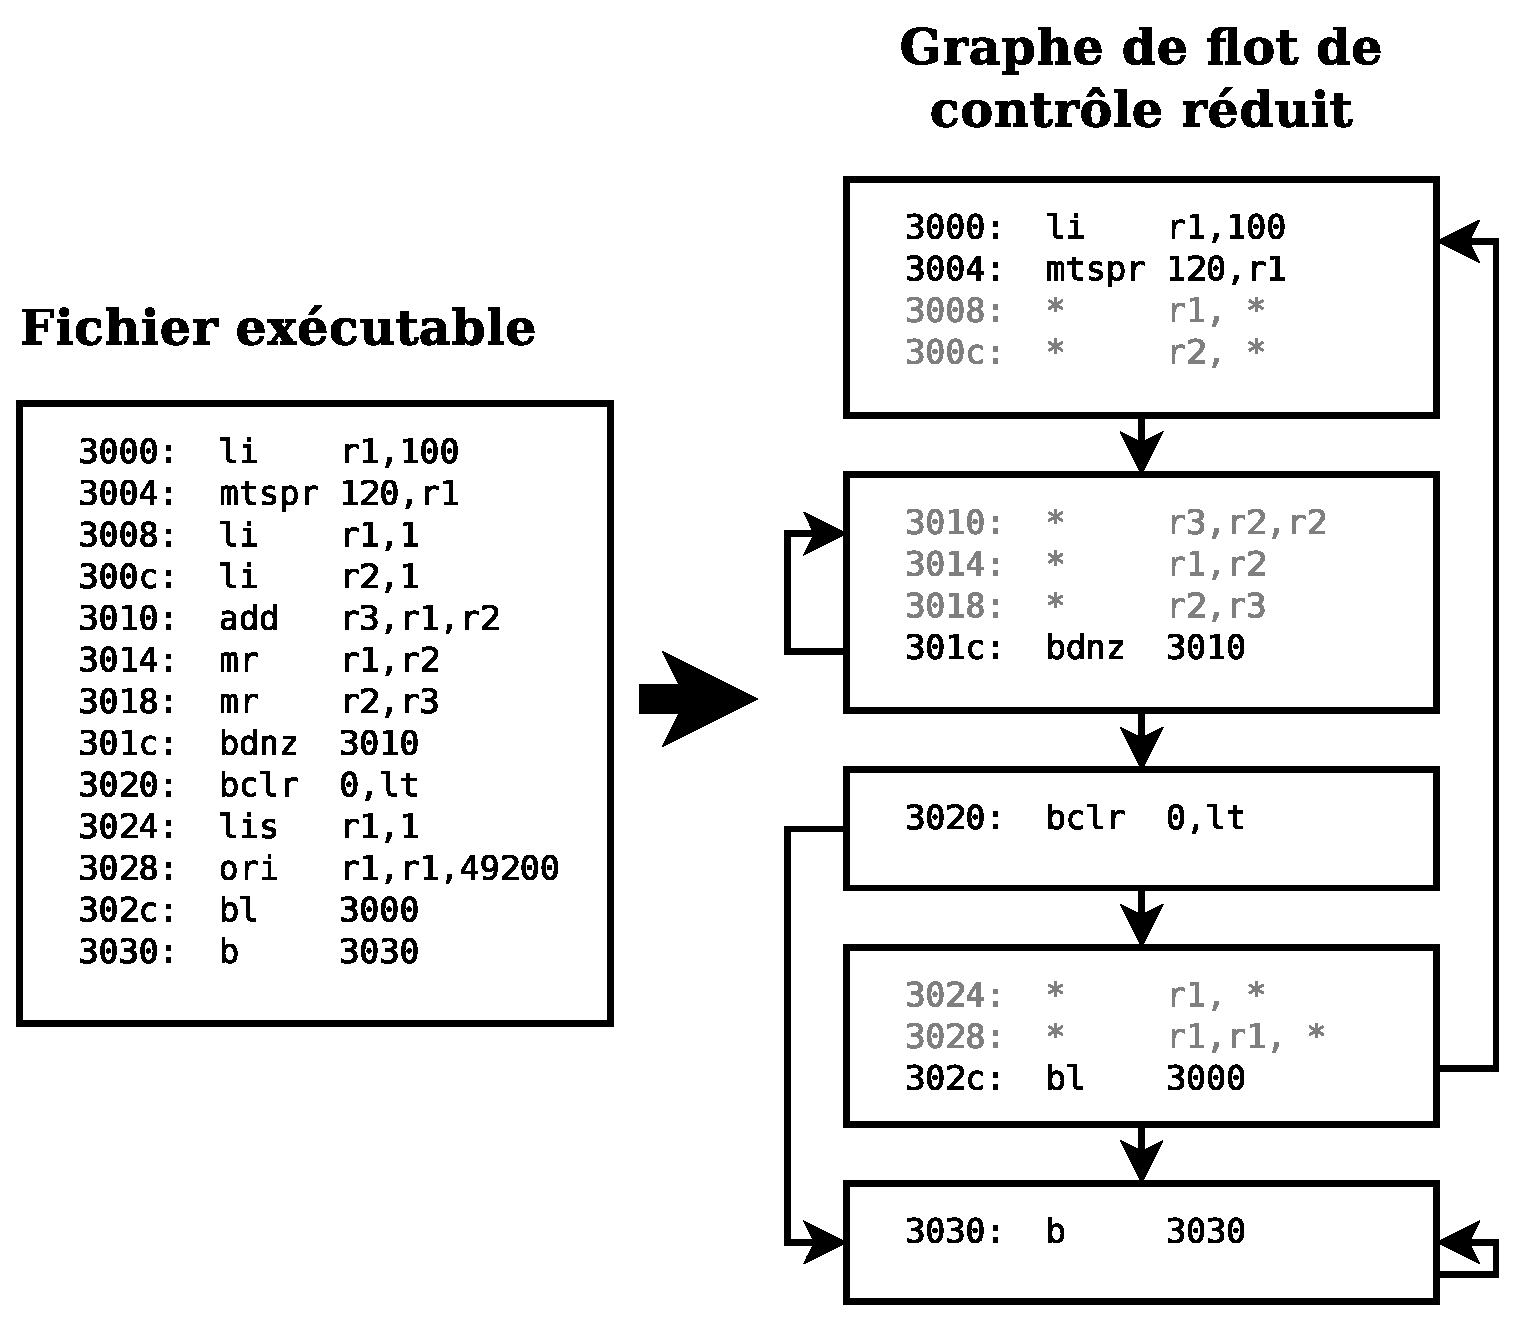
\includegraphics[scale=.3]{cfg.eps}
        \caption{Exemple schématique}
      \end{figure}
    \end{frame}
    
  %\begin{frame}\small
  %  \frametitle{Plan}
  %  \tableofcontents
  %\end{frame}

  \section{Implémentation}
    \begin{frame}\small
      \frametitle{\secname}
      %\framesubtitle{\subsecname}

      \begin{figure}
        \centering
        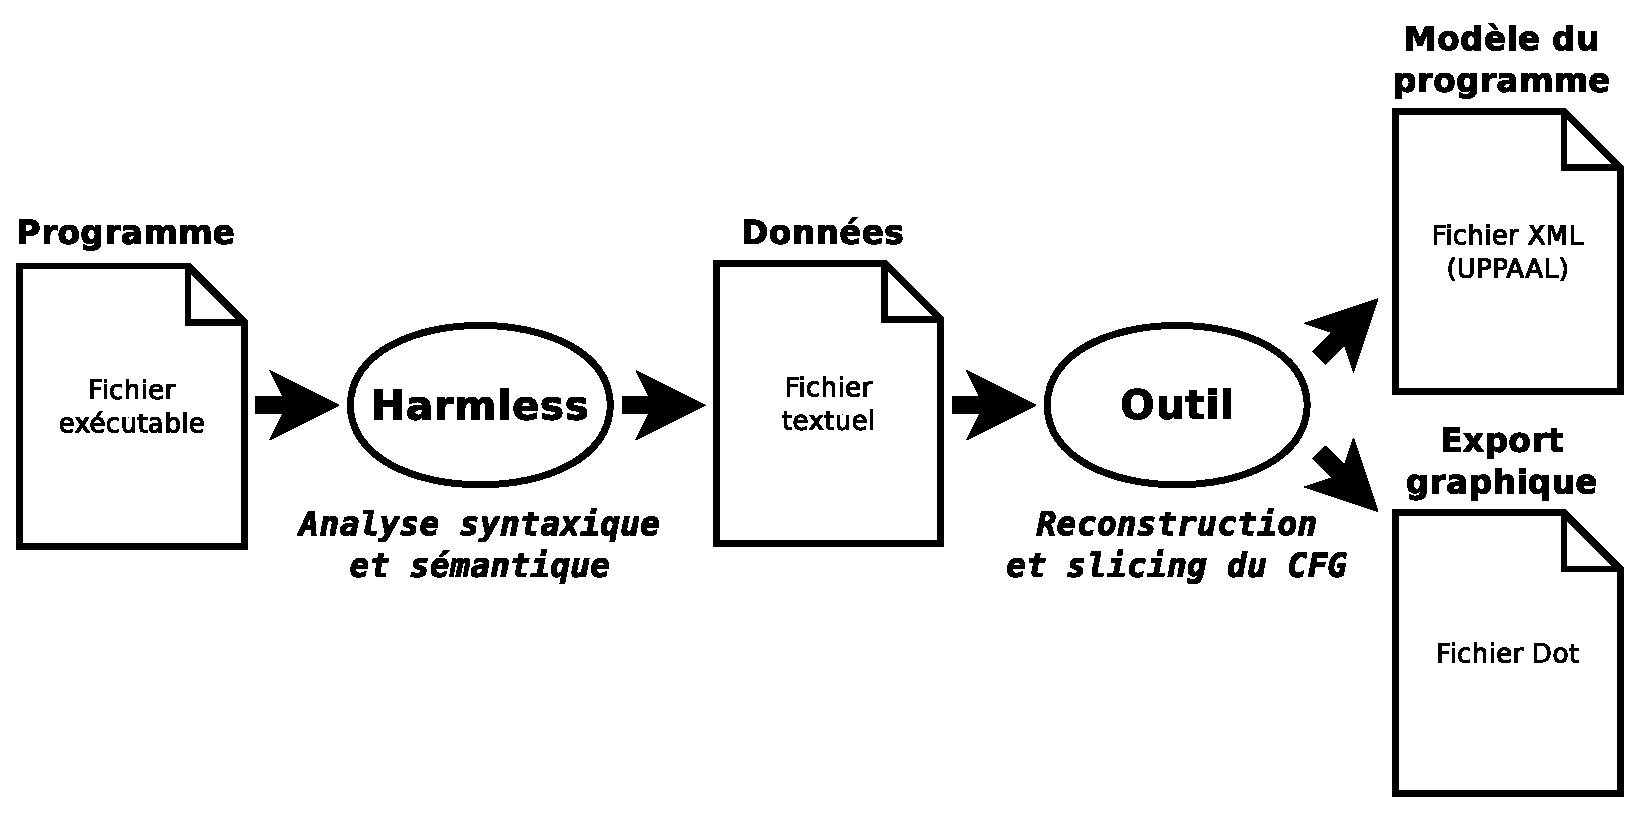
\includegraphics[scale=.3]{archi.eps}
        \caption{Architecture}
      \end{figure}

      \begin{description}
        \item[Harmless] Analyse sématique des fichiers exécutables
        \item[Haskell] Langage de programmation fonctionnel
        \item[Hoopl] Bibliothèque de manipulation de CFG
      \end{description}
    \end{frame}

  \section{Perspectives}
    \begin{frame}\small
      \frametitle{\secname}
      %\framesubtitle{\subsecname}

      \begin{itemize}
        \item Poursuite du travail sur l'outil
        \item Production d'un modèle du matériel multi-c{\oe}ur
        \item Exploration des possibilités de l'analyse temporelle par vérification de modèles
      \end{itemize}
    \end{frame}

\end{document}
